\documentclass{TDP003mall}

\usepackage{tabularx}
\usepackage{hyperref}
\usepackage{graphicx}
\usepackage{float}
\usepackage{listings}
\usepackage{amssymb}
\graphicspath{ {./images/} }
\usepackage{color}

\definecolor{mygreen}{rgb}{0,0.6,0}
\definecolor{mygray}{rgb}{0.5,0.5,0.5}
\definecolor{mymauve}{rgb}{0.58,0,0.82}

\lstset{
  backgroundcolor=\color{white},   % choose the background color; you must add \usepackage{color} or \usepackage{xcolor}; should come as last argument
  basicstyle=\footnotesize,        % the size of the fonts that are used for the code
  breakatwhitespace=false,         % sets if automatic breaks should only happen at whitespace
  breaklines=true,                 % sets automatic line breaking
  captionpos=b,                    % sets the caption-position to bottom
  commentstyle=\color{mygreen},    % comment style
  deletekeywords={...},            % if you want to delete keywords from the given language
  escapeinside={\%*}{*)},          % if you want to add LaTeX within your code
  extendedchars=true,              % lets you use non-ASCII characters; for 8-bits encodings only, does not work with UTF-8
  frame=single,	                   % adds a frame around the code
  keepspaces=true,                 % keeps spaces in text, useful for keeping indentation of code (possibly needs columns=flexible)
  keywordstyle=\color{red},       % keyword style
  language=Python,                 % the language of the code
  morekeywords={*,...,RotatingFieldHandler,handler,app,},            % if you want to add more keywords to the set
  numbers=left,                    % where to put the line-numbers; possible values are (none, left, right)
  numbersep=5pt,                   % how far the line-numbers are from the code
  numberstyle=\tiny\color{mygray}, % the style that is used for the line-numbers
  rulecolor=\color{black},         % if not set, the frame-color may be changed on line-breaks within not-black text (e.g. comments (green here))
  showspaces=false,                % show spaces everywhere adding particular underscores; it overrides 'showstringspaces'
  showstringspaces=false,          % underline spaces within strings only
  showtabs=false,                  % show tabs within strings adding particular underscores
  stepnumber=2,                    % the step between two line-numbers. If it's 1, each line will be numbered
  stringstyle=\color{mygreen},     % string literal style
  tabsize=2,	                   % sets default tabsize to 2 spaces
  title=\lstname                   % show the filename of files included with \lstinputlisting; also try caption instead of title
}

\newcommand{\version}{Version 1.0}
\author{Jimmie Roos, \url{jimro697@student.liu.se}\\
Sebastian Grunditz, \url{sebgr273@student.liu.se}}
\title{Systemdokumentation}
\date{2018-10-18}
\rhead{Jimmie Roos\\
Sebastian Grunditz}



\begin{document}
\projectpage
\tableofcontents
⁠\pagenumbering{gobble}
\thispagestyle{empty}
\newpage
\pagenumbering{arabic}
\section*{Revisionshistorik}
\begin{table}[!h]
\begin{tabularx}{\linewidth}{|l|X|l|}
\hline
Ver. & Revisionsbeskrivning & Datum \\\hline
1.0 & Första version & 18/10-18 \\\hline
1.1 & Revision efter kommentarer & 25/10-18 \\\hline
\end{tabularx}
\end{table}

\section{Introduktion}
\subsection{Datalagret}
Datalagret är utvecklat enligt kravspecifikationerna, som du kan hitta \href{https://www.ida.liu.se/~TDP003/current/portfolio-api_python3/}{här}. Vi har även skrivit tre hjälpfunktioner, \texttt{check\_search()} och \texttt{search\_project()}, för \texttt{search()}, och \texttt{get\_latest\_project()} för startsidan.
\subsubsection{Check\_search(search\_word, item\_)}
Det funktionen gör är att kolla om det sökord man får in, finns i projektet man vill kolla i. Den kallas på varje projekt i listan, men hanterar ett projekt i taget.
Funktionen har tre delar. Först kollar den om det man vill jämföra med sökordet är en integer. I sådant fall försöker den göra om sökordet till en integer, och om de stämmer
överens skickar den tillbaka \texttt{True}. Annars kollar den om vi vill kolla i en lista, och kör en koll rekursivt på varje del föremål i listan, bryter ifall den hittar det
den letar efter, och skickar tillbaka \texttt{True}.

Den sista delen antar att det vi söker i är en string. Då gör den om båda input så att de endast innehåller versaler, och kollar om sökordet finns i strängen vi söker i. Ifall den finns skickar den tillbaka \texttt{True}.
\subsubsection{Search\_project(project, search\_word, searchfield)}
Kollar först om det man söker på är en lista med saker eller inte. Om det är en lista så körs \texttt{check\_search()} på varje sökord och returnerar \texttt{True} om det stämmer.
Om det inte är en lista så körs \texttt{check\_search()} på det sökord man använde.

\subsubsection{Get\_latest\_project(db)}
Den här funktionen söker igenom listan, med hjälp av \texttt{search()} så att databasen kommer tillbaka, sorterad efter start datum. Sedan returnerar den det första elementet i listan, vilket motsvarar
senast påbörjade projekt.

\newpage
\section{Översikt}
\subsection{Översiktsbild}
\begin{figure}[H]
    \centering
    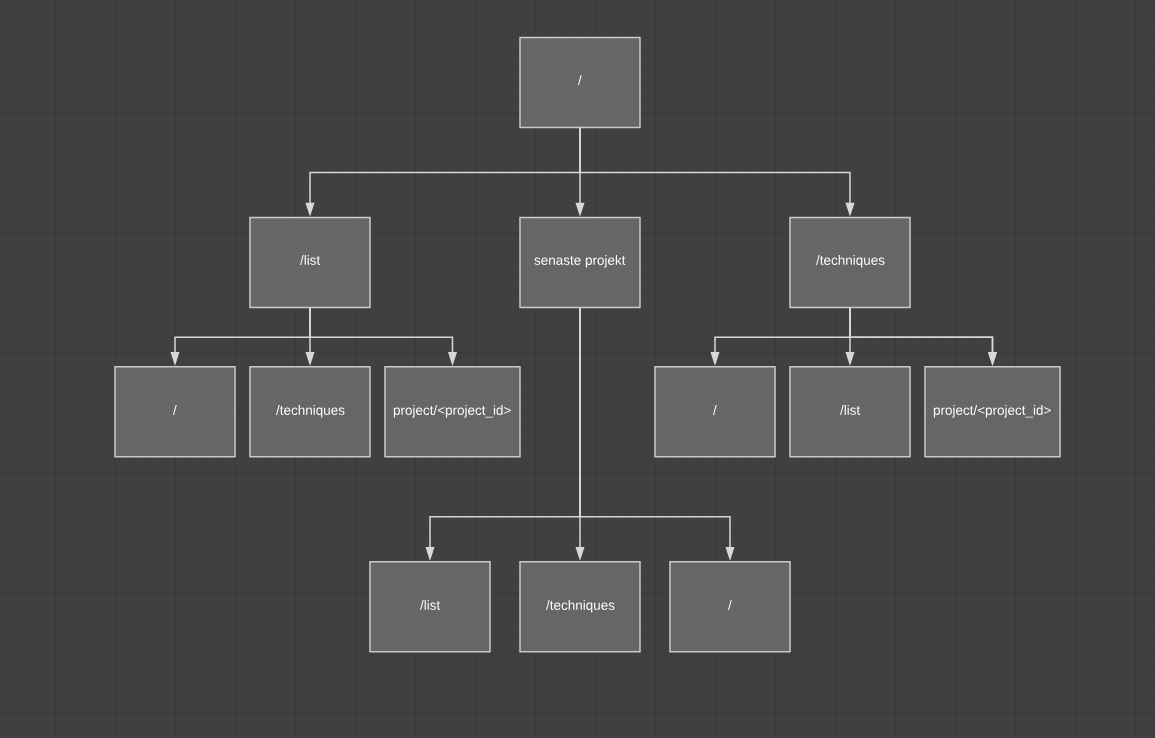
\includegraphics[width=\linewidth]{overview.PNG}
    \caption{Översiktsbild över hemsidan}
    \label{fig:overview}
\end{figure}
Figur \ref{fig:overview} visar ett enkelt flödesschema för navigering på hemsidan. ``Senaste projektet'' är isolerat, då det ligger på startsidan. Varje steg neråt i flödesschemat visar alla möjliga steg man kan ta från just den sidan.
\subsection{startsidan}
På indexsidan laddas det senaste projektet och visas på skärmen för användaren, tillsammans med information om den som äger hemsidan. Därifrån får man själv välja vad man vill ladda, t.ex projektsidan eller tekniksidan.
\subsection{söksidan}
Söksidan skriver ut alla projekt som stämmer in på sökkriterierna som skickats in från användaren. Ifall man blivit omdirigerad från en annan sida visar den alla projekt, sorterad i fallande ordning på start datum.
\subsection{Projektsida}
\begin{figure}[H]
    \centering
    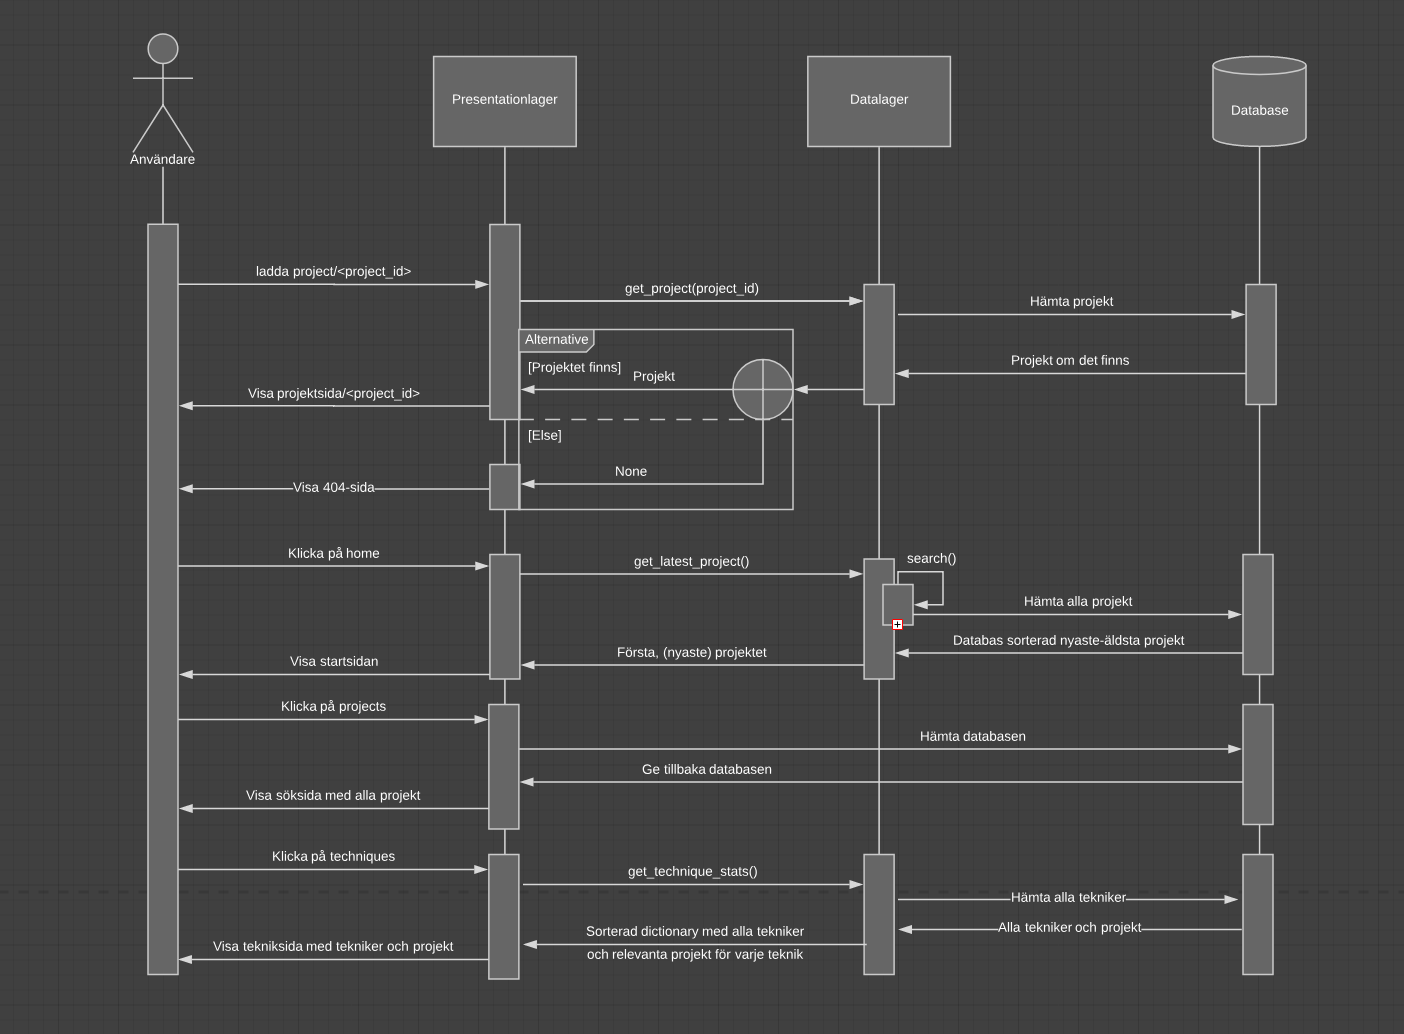
\includegraphics[width=\linewidth]{final.PNG}
    \caption{Sekvensdiagram för en projektsida. O med kryss i skickar vidare en av två möjliga output.}
    \label{fig:proj}
\end{figure}
Projektsidan laddar automatiskt projektet som användaren valde på förra sidan och skickar med bilder och beskrivningar, med mera, som hör till korresponderande projekt. Som syns i figur \ref{fig:proj} är det ett väldigt simpelt arbete för servern att ladda ``/list'', då den inte behöver interagera med datalagret. Detta beror på att vi skickar med hela databasen, som laddas under uppstart av servern, när man blir omdirigerad dit. 
\subsection{Tekniksidan}
Tekniksidan skriver ut alla tekniker som använts i projekten. Alla projekt delas sedan in i menyer för de tekniker som de har använt.
\newpage
\subsection{Filstruktur}
\begin{itemize}
    \item[$\bullet$] static
    \begin{itemize}
        \item[$\bullet$] images
        \begin{itemize}
            \item[--] *.jpg
            \item[--] *.png
            \item[--] *.tiff
        \end{itemize}
        \item[$\bullet$] style
        \begin{itemize}
            \item[--] *.css
        \end{itemize}
    \end{itemize}
    \item[$\bullet$] templates
    \begin{itemize}
        \item[--] *.html
        \item[--] *.json
        \item[--] *.xml
    \end{itemize}
    \item[--] *.py
    \item[--] *.md
    \item[--] database.json
    \item[--] app.py
    \item[--] datalayer.py
    \item[--] debug.log
\end{itemize}

\section{Presentationslagret}
I det här avsnittet beskrivs funktionerna i presentationslagret \path{app.py} mer ingående.
\subsection{page\_not\_found(error)}
\textbf{Metoder}
\begin{itemize}
    \item GET - Begär data från resurs.
\end{itemize}
\textbf{Parametrar}
\begin{itemize}
    \item error(error code) - Ett felmeddelande.
\end{itemize}
\textbf{Returns: render}
\begin{itemize}
    \item[] Redirect till 404-sidan.
\end{itemize}
Returnerar en 404-sida när vi får en 404 error.

\subsection{index()}
\textbf{Metoder}
\begin{itemize}
    \item GET - Begär data från resurs.
\end{itemize}
\textbf{Parametrar}
\begin{itemize}
    \item Inga.
\end{itemize}
\textbf{Returns: render}
\begin{itemize}
    \item[] Redirect till index.html.
\end{itemize}
Returnerar hemsidan, med senaste projektet.

\subsection{search()}
\textbf{Metoder}
\begin{itemize}
    \item GET - Begär data från resurs.
    \item POST - Skicka data till servern för att skapa eller uppdatera en resurs.
\end{itemize}
\textbf{Parametrar}
\begin{itemize}
    \item Inga.
\end{itemize}
\textbf{Returns: render}
\begin{itemize}
    \item[] Returnar en lista med sökresultat.
\end{itemize}
Om vi får en GET så returnerar vi hela databasen.
Om vi får en POST så filtrerar vi databasen baserat på input av användaren.

\subsection{techniques()}
\textbf{Metoder}
\begin{itemize}
    \item GET - Begär data från resurs.
\end{itemize}
\textbf{Parametrar}
\begin{itemize}
    \item Inga.
\end{itemize}
\textbf{Returns: render}
\begin{itemize}
    \item[] Redirect till techniques.
\end{itemize}

\subsection{project(project\_id)}
\textbf{Metoder}
\begin{itemize}
    \item GET - Begär data från resurs.
\end{itemize}
\textbf{Parametrar}
\begin{itemize}
    \item project\_id(integer) - För att beskriva vilket projekt sidan handlar om.
\end{itemize}
\textbf{Returns: render}
\begin{itemize}
    \item[] Redirect till projektsida eller 404.
\end{itemize}
Returnerar en sida med specifikt projekt eller 404 om inte projektet hittas.
\newpage
\subsection{list()}
\textbf{Metoder}
\begin{itemize}
    \item GET - Begär data från resurs.
\end{itemize}
\textbf{Parametrar}
\begin{itemize}
    \item Inga.
\end{itemize}
\textbf{Returns: render}
\begin{itemize}
    \item[] Redirect till söksida med resultat.
\end{itemize}
Får in databasen, representerad av en dictionary. Skickar tillbaka en söksida med alla projekt om inget söks efter, eller om man kommer till ``/list'' från en annan sida. Returnerar söksidan med filtrerat resultat om användaren har sökt på något specifikt.


\section{Felsökning}
Vi använde oss av en funktion som heter RotatingFileHandler för att kunna skriva ut errormeddelanden till fil.
Vid en error så skickas användaren till en 404-sida och felmeddelandena skrivs ut till en fil \path{debug.log} i projektmappen.
Den skriver felmeddelande på en \textit{DEBUG}-nivå, vilket innebär att den skriver ut information som är användbar vid debugging
av hemsidan. För att inte \path{debug.log} ska bli allt för stor, har den en max byte-gräns, innan den stänger och sparar loggen, för att öppna en ny.
Den sparar de fem senaste dokumenten, vilket innebär att totalt sparar den 60000 bytes med log från hemsidan. Om man vill ändra, gör man det i app.py på följande ställe:
\begin{lstlisting}
if __name__ == "__main__":
    handler = RotatingFileHandler('debug.log', maxBytes=10000, backupCount=5)
    handler.setLevel(logging.DEBUG)
    app.logger.addHandler(handler)
    app.run(debug=True)
\end{lstlisting}
I \texttt{RotatingFileHandler()} ändrar man på \textit{maxBytes} för att ändra storleken på \path{.log}-filen och \textit{backupCount} för att ändra antalet \path{.log}-filer som sparas.


För att prova om datalagret fungerar så har vi en \path{data_test.py} som vi kör på \path{data.json} och ser om vi får några fel.
Båda dessa finns att hämta på \href{https://gitlab.ida.liu.se/filst04/tdp003-2018-database-tests.git}{gitlab}.
\newpage
\section{Appendix}
\begin{appendix}
  \listoffigures
\end{appendix}
\end{document}
